\documentclass[final,3p]{elsarticle}

\usepackage{amsmath,amssymb,bm}
\usepackage{graphicx}
\usepackage{booktabs}
%\usepackage{hyperref}  % Disabled: causes TeX capacity overflow with many H-floats
%\usepackage{lineno}
\usepackage{float}
\usepackage{multirow}
\usepackage[titletoc]{appendix}
\usepackage{tikz}
\usetikzlibrary{arrows.meta,positioning,shapes.geometric}

\newcommand{\vect}[1]{\boldsymbol{#1}}
\newcommand{\mat}[1]{\mathbf{#1}}

\graphicspath{{../figures/}{../results/}{../results/elliptic/}{../results/benchmark/}{../results/3d_tumble_scenario2/}}

\journal{Acta Astronautica}

\begin{document}

\begin{frontmatter}

\title{Hierarchical Reachability Certification for MPC-Guided Approach to a Tumbling Target Under Rotating Line-of-Sight Constraints}

\author[aff1]{Omer Burak Iskender\corref{cor1}}
\ead{iske0001@e.ntu.edu.sg}

\cortext[cor1]{Corresponding author}
\affiliation[aff1]{organization={School of Electrical and Electronic Engineering, Nanyang Technological University},
  city={Singapore}, country={Singapore}}

\begin{abstract}
Autonomous proximity operations with tumbling, uncooperative spacecraft require guidance systems that can certify the feasibility of approach trajectories before execution.  When the target tumbles, its body-fixed docking corridor rotates in the chaser's coordinate frame, producing time-varying polyhedral constraints whose feasibility depends critically on the interplay between tumble rate and thrust authority.  This paper develops a hierarchical reachability framework that computes three nested analytical safe-start sets with progressively stronger guarantees---nominal ($\mathcal{X}_{\mathrm{nom}}$), stochastic ($\mathcal{X}_{\mathrm{stoch}}$, 95\% confidence), and robust ($\mathcal{X}_{\mathrm{rob}}$, bounded disturbances)---satisfying $\mathcal{X}_{\mathrm{rob}} \subseteq \mathcal{X}_{\mathrm{stoch}} \subseteq \mathcal{X}_{\mathrm{nom}}$ by construction.  An independent Monte~Carlo campaign ($\mathcal{X}_{\mathrm{MC}}$) provides empirical closed-loop validation under nonlinear two-body-plus-$J_2$ truth dynamics coupled to a receding-horizon quadratic-program (QP) controller with state-tracking, input-rate, and terminal penalties.  A parametric sweep over tumble rates 1--5~deg/s and thrust authorities 0.02--0.20~m/s$^2$ on a $300\!\times\!300$ evaluation grid (i)~identifies $a_{\max}/\omega_t^2$ as the single dimensionless parameter governing approach feasibility, (ii)~confirms the analytical hierarchy $\mathcal{X}_{\mathrm{rob}} \subseteq \mathcal{X}_{\mathrm{stoch}} \subseteq \mathcal{X}_{\mathrm{nom}}$ across all 20 parameter combinations with zero point-wise violations, (iii)~shows that analytical certification completes in 53~s versus 2--4~hours for Monte~Carlo, enabling on-board mission replanning, and (iv)~validates the architecture under full three-dimensional tumbling with Euler dynamics and intermediate-axis instability, achieving zero corridor violations despite $120^\circ$ spin-axis precession.
\end{abstract}

\begin{keyword}
spacecraft rendezvous \sep uncooperative target \sep reachability analysis \sep time-varying constraints \sep model predictive control \sep line-of-sight corridor \sep feasibility certification
\end{keyword}

\end{frontmatter}

%\linenumbers  % Disabled: causes TeX capacity overflow with many figures

%% ========================================================================
\section{Introduction}
\label{sec:intro}
%% ========================================================================

On-orbit servicing, active debris removal, and inspection missions increasingly require autonomous rendezvous and proximity operations with uncooperative, potentially tumbling targets~\cite{Flores2014,Fehse2003,Bonnal2013}.  Unlike cooperative docking where the target maintains a stable attitude and provides relative navigation aids, uncooperative scenarios demand that the chaser autonomously satisfy safety constraints defined relative to a rotating target body frame~\cite{Woffinden2007,Aghili2012}.

When the target tumbles, its body-fixed docking corridor---a polyhedral line-of-sight (LOS) cone---rotates in the chaser's local-vertical local-horizontal (LVLH) frame.  This rotation transforms a static constraint into a time-varying one whose feasibility depends on the ratio of the chaser's thrust authority to the square of the target's tumble rate.  A chaser position that lies inside the LOS cone at one instant may violate it moments later unless the chaser can co-rotate with sufficient control authority.

The central question motivating this work is: \emph{given the target's tumble rate $\omega_t$ and the chaser's maximum thrust-to-mass ratio $a_{\max}$, from which initial positions can the chaser safely approach while maintaining LOS constraint satisfaction at all times?}  Answering this question requires computing the safe-start region---the set of initial conditions from which constraint-satisfying trajectories exist~\cite{Blanchini2008}.  Because the answer depends on disturbance assumptions, we seek not a single region but a \emph{hierarchy} of nested regions providing progressively stronger guarantees.

\subsection{Related Work}

\paragraph{Relative dynamics and MPC for proximity operations.}
Linearised relative motion using the Hill-Clohessy-Wiltshire (HCW/CWH) equations~\cite{Hill1878,Clohessy1960} provides the standard prediction model for proximity guidance~\cite{Schaub2018}.  Model predictive control (MPC) has been widely applied to spacecraft rendezvous~\cite{Mayne2000,Rawlings2017,Weiss2015,Zagaris2018}, typically with static or slowly varying keep-out-zone constraints.  Richards et al.~\cite{Richards2002} formulated avoidance-constrained trajectory planning as a mixed-integer linear program.  Jewison et al.~\cite{Jewison2016} used MPC with ellipsoidal obstacle constraints.  Breger and How~\cite{Breger2008} developed safe trajectory planning for autonomous rendezvous.

\paragraph{Tumbling target guidance.}
For tumbling targets, Virgili-Llop et al.~\cite{Virgili2019} developed convex-programming guidance for robotic-arm capture.  Aghili~\cite{Aghili2012} addressed visually guided capture with uncertain dynamics.  Di~Mauro et al.~\cite{DiMauro2018} applied differential algebra for nonlinear proximity control, and Grzymisch and Fichter~\cite{Grzymisch2015} derived analytic optimal control for approach to a tumbling target.  Zappulla et al.~\cite{Zappulla2017} used artificial potential fields for real-time proximity manoeuvres.  These works focus on trajectory generation or capture, not on systematic pre-mission feasibility certification of the approach region.

\paragraph{Reachability and set-theoretic methods.}
Set-theoretic methods~\cite{Blanchini2008,Blanchini1999} and Hamilton-Jacobi approaches~\cite{Mitchell2005,Bansal2017} provide frameworks for computing safe operating regions.  Chance-constrained approaches~\cite{Blackmore2011,Mesbah2016} provide probabilistic guarantees.  Bonalli et al.~\cite{Bonalli2019} developed sequential convex programming with guaranteed convergence for constrained trajectory optimisation.

\paragraph{Tube-based robust MPC for proximity operations.}
Tube-based MPC~\cite{Langson2004,Rakovic2005} tightens constraints using minimal robust positively invariant (mRPI) sets to guarantee constraint satisfaction under bounded disturbances.  Mammarella et al.~\cite{Mammarella2020} applied tube-based robust MPC to spacecraft proximity operations, demonstrating experimental validation on a floating platform.  Dong et al.~\cite{Dong2020} extended this to a tumbling target with output-feedback estimation, using approach corridor constraints in LVLH.  Specht et al.~\cite{Specht2023} developed a full TRACE pipeline (estimation, planning, tube MPC tracking) for free-tumbling debris capture.  Leomanni et al.~\cite{Leomanni2022} introduced variable-horizon MPC for tumbling-target rendezvous, later extended with robust tube guarantees~\cite{Quartullo2024}.  Di~Cairano et al.~\cite{DiCairano2012} formulated MPC with LOS cone constraints for rotating platforms but without tube-based robustness.  These works embed robustness within the MPC via constraint tightening but do not provide a separate, hierarchical pre-mission feasibility certification layer.

\paragraph{Reachability-guaranteed control for dynamic targets.}
Faraci and Lampariello~\cite{Faraci2025} recently addressed the complementary problem of \emph{guaranteed reachability}: ensuring that the chaser \emph{can reach} all possible target orientations at a terminal time, solved via nonlinear programming with guaranteed reachability (GRP) constraints.  Their formulation guarantees that the chaser's reachable set encloses the target's orientation envelope, but does not certify corridor constraint satisfaction during the approach.

\paragraph{Gap.}
No existing work provides a unified, computationally efficient framework that maps the entire approach region into nested feasibility sets for a tumbling target with rotating polyhedral constraints under nominal, stochastic, and robust assumptions simultaneously.  Tube-based MPC methods tighten constraints within the controller but do not produce an explicit pre-mission map of the feasible approach region.  Reachability-guaranteed methods certify terminal interception but not corridor safety during transit.

\subsection{Contributions}

This paper makes four specific contributions:
\begin{enumerate}
\item \textbf{Hierarchical feasibility certification.}  Three nested analytical safe-start regions---robust ($\mathcal{X}_{\mathrm{rob}}$), stochastic ($\mathcal{X}_{\mathrm{stoch}}$), and nominal ($\mathcal{X}_{\mathrm{nom}}$)---are defined and proven to satisfy $\mathcal{X}_{\mathrm{rob}} \subseteq \mathcal{X}_{\mathrm{stoch}} \subseteq \mathcal{X}_{\mathrm{nom}}$ by construction.  An independent empirical Monte~Carlo set ($\mathcal{X}_{\mathrm{MC}}$) provides closed-loop validation under the actual MPC controller.

\item \textbf{Directional per-constraint erosion with synchronisation bound.}  A closed-form inner approximation of the nominal safe region is derived using the constraint-slack rate induced by body-frame rotation and a range-dependent synchronisation limit $r_{\mathrm{sync}} = 2a_{\max}/\omega_t^2$.

\item \textbf{Identification of $a_{\max}/\omega_t^2$ as the universal scaling parameter.}  Through dimensional analysis and parametric sweeps, the ratio $a_{\max}/\omega_t^2$ is shown to collapse all safe-fraction results onto a single curve.

\item \textbf{Physically honest closed-loop validation.}  Truth propagation uses full nonlinear two-body-plus-$J_2$ dynamics, demonstrating that double-integrator truth models produce artificially successful approaches through unphysical state teleportation.
\end{enumerate}

\subsection{Paper Organisation}

Section~\ref{sec:mission} defines the mission scenario.  Section~\ref{sec:frames} establishes reference frames.  Section~\ref{sec:dynamics} presents the dynamics.  Section~\ref{sec:los} formulates the LOS corridor.  Section~\ref{sec:problem} states the MPC problem.  Section~\ref{sec:reachability} develops safe-start region analysis.  Section~\ref{sec:mc} details Monte~Carlo validation.  Section~\ref{sec:results} presents results.  Section~\ref{sec:discussion} discusses findings---including extension to full 3D tumbling with Euler dynamics (Section~\ref{sec:3d_tumble})---and Section~\ref{sec:conclusions} concludes.


%% ========================================================================
\section{Mission Scenario}
\label{sec:mission}
%% ========================================================================

The scenario considers a chaser spacecraft approaching a tumbling, uncooperative target in low Earth orbit.  Table~\ref{tab:mission} summarises the parameters.

\begin{table}[H]
\centering
\caption{Mission scenario parameters.}
\label{tab:mission}
\begin{tabular}{lll}
\toprule
\textbf{Parameter} & \textbf{Value} & \textbf{Description} \\
\midrule
\multicolumn{3}{l}{\emph{Orbit}} \\
$\mu$ & $3.986 \times 10^{14}$ m$^3$/s$^2$ & Gravitational parameter \\
Altitude & 500 km & Circular LEO \\
$n$ & $1.131 \times 10^{-3}$ rad/s & Mean motion \\
$J_2$ & $1.083 \times 10^{-3}$ & Zonal harmonic \\
\midrule
\multicolumn{3}{l}{\emph{Target}} \\
$\omega_t$ & $\{1,2,3,4,5\}$ deg/s & Tumble rate about body $z$ \\
\midrule
\multicolumn{3}{l}{\emph{Chaser}} \\
$a_{\max}$ & $\{0.20, 0.10, 0.05, 0.02\}$ m/s$^2$ & Max thrust-to-mass ratio \\
$\mathbf{r}_0$ & $[0, 200, 0]^\top$ m (LVLH) & Nominal initial position \\
\midrule
\multicolumn{3}{l}{\emph{Docking corridor}} \\
$\alpha_c$ & 30$^\circ$ & LOS cone half-angle \\
$n_f$ & 8 & Polyhedral cone faces \\
$y_{\min}$ & 1.0 m & Corridor floor distance \\
\midrule
\multicolumn{3}{l}{\emph{Simulation}} \\
$T_{\mathrm{sim}}$ & 400--600 s & Duration \\
$\Delta t$ & 1.0 s & Control time step \\
\bottomrule
\end{tabular}
\end{table}


%% ========================================================================
\section{Reference Frame Definitions}
\label{sec:frames}
%% ========================================================================

Three coordinate frames are employed.

\paragraph{Earth-Centred Inertial (ECI) Frame $\mathcal{F}_I$.}
Origin at Earth's centre; $\hat{\mathbf{x}}_I$ toward the vernal equinox, $\hat{\mathbf{z}}_I$ along Earth's spin axis, $\hat{\mathbf{y}}_I$ completing the right-hand triad.

\paragraph{Local Vertical Local Horizontal (LVLH) Frame $\mathcal{F}_L$.}
Centred on the target, with axes:
\begin{equation}
\hat{\mathbf{x}}_L = \frac{\mathbf{r}_t}{\|\mathbf{r}_t\|}, \quad
\hat{\mathbf{z}}_L = \frac{\mathbf{r}_t \times \mathbf{v}_t}{\|\mathbf{r}_t \times \mathbf{v}_t\|}, \quad
\hat{\mathbf{y}}_L = \hat{\mathbf{z}}_L \times \hat{\mathbf{x}}_L,
\label{eq:lvlh_def}
\end{equation}
so $x_L$ is radially outward, $y_L$ approximately along-track, and $z_L$ orbit-normal.  $R_{IL}$ maps $\mathcal{F}_L$ vectors to~$\mathcal{F}_I$.  Figure~\ref{fig:traj_2d} shows a representative approach trajectory projected onto the $x$--$y$ plane in both $\mathcal{F}_B$ and $\mathcal{F}_L$, and Figure~\ref{fig:traj_3d} shows the three-dimensional view in $\mathcal{F}_B$.

\paragraph{Target Body Frame $\mathcal{F}_B$.}
Fixed to the tumbling target with $+y_B$ along the docking axis.  Orientation relative to $\mathcal{F}_I$ is tracked by the unit quaternion $\mathbf{q}_{IB}$ (scalar-first), propagated via:
\begin{equation}
\dot{\mathbf{q}}_{IB} = \tfrac{1}{2}\,\mathbf{q}_{IB} \otimes [0;\; \boldsymbol{\omega}_B], \quad \boldsymbol{\omega}_B = [0, 0, \omega_t]^\top.
\label{eq:quat_prop}
\end{equation}

\begin{figure}[H]
\centering
\includegraphics[width=0.48\textwidth]{fig_2d_xy_tb.png}%
\hfill%
\includegraphics[width=0.48\textwidth]{fig_2d_xy_lvlh.png}
\caption{Representative approach trajectory projected onto the $x$--$y$ plane.  \textbf{Left:} target body frame $\mathcal{F}_B$.  The chaser starts at 200~m along the docking axis ($+y_B$) and descends within the body-fixed LOS cone (orange), reaching the hold point near the origin.  The trajectory remains centred on the docking axis throughout.  \textbf{Right:} LVLH frame $\mathcal{F}_L$.  The same trajectory appears as a large spiral because the cone rotates with the tumbling target; CWH along-track drift produces the characteristic radial excursion before the controller captures the hold.}
\label{fig:traj_2d}
\end{figure}

\begin{figure}[H]
\centering
\includegraphics[width=0.65\textwidth]{fig_3d_target_body.png}
\caption{Three-dimensional approach trajectory in the target body frame $\mathcal{F}_B$.  The polyhedral LOS cone (orange wireframe, 8 faces, half-angle $30^\circ$) is body-fixed.  The chaser (blue curve) enters the cone from 200~m, manoeuvres onto the docking axis ($+y_B$), and converges to the hold point (black star) while remaining within the cone at all times.  The out-of-plane ($z_B$) motion is negligible because the tumble axis is aligned with $z$.}
\label{fig:traj_3d}
\end{figure}


%% ========================================================================
\section{Dynamics Model}
\label{sec:dynamics}
%% ========================================================================

\subsection{Nonlinear Truth Model}
\label{sec:truth}

Truth propagation uses full nonlinear dynamics in $\mathcal{F}_I$.  Each spacecraft is governed by:
\begin{equation}
\ddot{\mathbf{r}}_I = -\frac{\mu}{\|\mathbf{r}_I\|^3}\,\mathbf{r}_I + \mathbf{a}_{J_2}(\mathbf{r}_I) + \mathbf{a}_{\mathrm{ctrl}},
\label{eq:eci_eom}
\end{equation}
where the $J_2$ perturbation is:
\begin{equation}
\mathbf{a}_{J_2} = -\frac{3J_2\mu R_e^2}{2\|\mathbf{r}_I\|^5}
\begin{bmatrix}
x_I(1 - 5z_I^2/\|\mathbf{r}_I\|^2) \\
y_I(1 - 5z_I^2/\|\mathbf{r}_I\|^2) \\
z_I(3 - 5z_I^2/\|\mathbf{r}_I\|^2)
\end{bmatrix}.
\label{eq:J2}
\end{equation}
Integration uses \texttt{ode113} with relative tolerance $10^{-10}$ and absolute tolerance $10^{-12}$.  Target and chaser are propagated independently in $\mathcal{F}_I$; the relative state is computed by frame transformation at each step.

\subsection{CWH Prediction Model}

The MPC prediction model uses the CWH equations~\cite{Clohessy1960} for linearised relative motion about a circular orbit:
\begin{align}
\ddot{x} &= 3n^2 x + 2n\dot{y} + a_x, \notag \\
\ddot{y} &= -2n\dot{x} + a_y, \label{eq:cwh} \\
\ddot{z} &= -n^2 z + a_z. \notag
\end{align}

In discrete time with $\mathbf{x} = [x, y, z, \dot{x}, \dot{y}, \dot{z}]^\top$:
\begin{equation}
\mathbf{x}_{k+1} = \Phi(\Delta t)\,\mathbf{x}_k + B_d(\Delta t)\,\mathbf{u}_k + \mathbf{w}_k,
\label{eq:discrete}
\end{equation}
where $\Phi(\tau)$ is the exact state-transition matrix (Appendix~\ref{app:stm}).  The $(2,1)$ element $6(\sin n\tau - n\tau)$ produces secular along-track drift proportional to radial offset---a critical coupling absent in double-integrator models.

\subsection{Frame Transformations}

The relative state in $\mathcal{F}_B$ is:
\begin{align}
\mathbf{r}_B &= R_{IB}^\top(\mathbf{r}_c - \mathbf{r}_t), \label{eq:pos_transform} \\
\mathbf{v}_B &= R_{IB}^\top(\mathbf{v}_c - \mathbf{v}_t) - \boldsymbol{\omega}_B \times \mathbf{r}_B, \label{eq:vel_transform}
\end{align}
where the transport term in~\eqref{eq:vel_transform} requires co-rotation velocity $v_{\mathrm{corot}} = \omega_t r$ at range $r$.

\subsection{Online MPC Linearisation}
\label{sec:linearise}

At every control step $k$, the MPC prediction matrices $(A_{d,k}, B_{d,k})$ are recomputed via forward finite differences ($\epsilon = 10^{-6}$) applied to the full nonlinear propagation pipeline:
\begin{equation}
\underbrace{\mathcal{F}_B \to \text{ECI}}_{\text{frame recovery}} \to
\underbrace{\texttt{ode113}}_{\substack{\text{two-body}\\\text{+}J_2}} \to
\underbrace{\text{attitude}}_{\text{update}} \to
\underbrace{\text{ECI} \to \mathcal{F}_B}_{\substack{\text{body-frame}\\\text{projection}}}
\label{eq:linearise_pipeline}
\end{equation}
Each column of $A_{d,k}$ (respectively $B_{d,k}$) is obtained by perturbing one state (respectively input) component by $\epsilon$ and differencing the output of this pipeline, requiring $1 + n_x + n_u = 10$ nonlinear propagations per step.  The resulting time-varying matrices capture $J_2$ secular drift, Coriolis coupling, and the instantaneous attitude geometry---effects that a frozen CWH model cannot represent.

\paragraph{Model usage distinction.}
The CWH state-transition matrix $\Phi(\tau)$ (Appendix~\ref{app:stm}) is used exclusively for the \emph{offline} reachability analysis of Section~\ref{sec:reachability}, where its closed-form structure enables efficient polytope computations.  All \emph{online} MPC predictions use the finite-difference linearisation described above, ensuring that the controller's prediction model is consistent with the nonlinear truth dynamics.


%% ========================================================================
\section{Time-Varying LOS Corridor}
\label{sec:los}
%% ========================================================================

The docking corridor is a polyhedral cone in $\mathcal{F}_B$ with axis $+y_B$, half-angle $\alpha_c = 30^\circ$, approximated by $n_f = 8$ half-spaces plus a floor:
\begin{equation}
A_c\,\mathbf{p}_B \le b_c, \quad A_c \in \mathbb{R}^{9 \times 3}.
\label{eq:los_3d}
\end{equation}
The $i$-th face constraint is $\cos(\theta_i)\,x_B + \sin(\theta_i)\,z_B \le \tan(\alpha_c)\,y_B$ with $\theta_i = 2\pi(i-1)/n_f$, and the floor is $y_B \ge y_{\min}$.  In LVLH:
\begin{equation}
A_c\,R_z(-\omega_t t)\,\mathbf{p}_L \le b_c.
\label{eq:los_lvlh}
\end{equation}
Since the MPC operates in $\mathcal{F}_B$, constraints~\eqref{eq:los_3d} are time-invariant within the QP.


%% ========================================================================
\section{Problem Formulation}
\label{sec:problem}
%% ========================================================================

At each control step, the MPC solves over a receding horizon of $N_p$ steps:
\begin{subequations}
\label{eq:mpc}
\begin{align}
\min_{\mathbf{u}_{0:N_p\!-\!1}} \; J &= \sum_{j=0}^{N_p-1}\!\Big[ \|\hat{\mathbf{x}}_j - \mathbf{x}^{\mathrm{ref}}\|_Q^2 + \|\mathbf{u}_j\|_{R_u}^2 + \|\Delta\mathbf{u}_j\|_{R_{\Delta u}}^2 \Big] + \|\hat{\mathbf{x}}_{N_p} - \mathbf{x}^{\mathrm{ref}}\|_{Q_N}^2 \label{eq:cost} \\
\text{s.t.} \quad & \hat{\mathbf{x}}_{j+1} = A_d\,\hat{\mathbf{x}}_j + B_d\,\mathbf{u}_j, & j &= 0,\ldots,N_p\!-\!1, \label{eq:dyn_con} \\
& \hat{\mathbf{x}}_0 = \mathbf{x}_k, \label{eq:ic_con} \\
& A_c\,[\hat{\mathbf{x}}_j]_{1:3} \le b_c, & j &= 0,\ldots,N_p, \label{eq:los_con} \\
& -a_{\max}\mathbf{1} \le \mathbf{u}_j \le a_{\max}\mathbf{1}, & j &= 0,\ldots,N_p\!-\!1, \label{eq:input_con}
\end{align}
\end{subequations}
where $\Delta\mathbf{u}_j = \mathbf{u}_j - \mathbf{u}_{j-1}$ (with $\mathbf{u}_{-1}$ the previously applied input), and:
\begin{itemize}
\item $Q = \mathrm{diag}(15, 30, 15, 1, 1, 1)$: state deviation penalty (heavier on docking-axis);
\item $Q_N = 30Q$: terminal penalty;
\item $R_u = 10^{-2}I_3$: input regularisation;
\item $R_{\Delta u}$: input-rate penalty for smooth thrusting.
\end{itemize}

The reference $\mathbf{x}^{\mathrm{ref}} = [0, y_{\mathrm{ref}}(t), 0, 0, 0, 0]^\top$ tracks an exponentially decaying hold point: $y_{\mathrm{ref}}(t) = y_{\mathrm{end}} + (y_0 - y_{\mathrm{end}})e^{-t/\tau}$.  The QP is solved by OSQP~\cite{Stellato2020} with warm-starting and polishing; only $\mathbf{u}_0^*$ is applied (receding horizon).

\paragraph{Configuration variants.}  Two MPC configurations are used (Table~\ref{tab:mpc_config}).

\begin{table}[H]
\centering
\caption{MPC configurations for single-scenario and Monte~Carlo simulations.}
\label{tab:mpc_config}
\begin{tabular}{l c c}
\toprule
 & \textbf{Single scenario} & \textbf{Monte Carlo} \\
\midrule
$N_p$ & 40 & 20 \\
$R_{\Delta u}$ & $10^4 I_3$ & $\mathrm{diag}(10^5, 10^4, 10^5)$ \\
$T_{\mathrm{sim}}$ & 600 s & 400 s \\
OSQP max iter & 20\,000 & 5\,000 \\
ODE tolerances & $10^{-10}$/$10^{-12}$ & $10^{-8}$/$10^{-10}$ \\
\bottomrule
\end{tabular}
\end{table}

The MC configuration uses asymmetric $R_{\Delta u}$ (heavier penalty on radial/cross-track input rates) and shorter horizon to balance fidelity with computational cost across 3\,900 simulations.


%% ========================================================================
\section{Guidance Architecture}
\label{sec:guidance}
%% ========================================================================

The guidance system is a single receding-horizon MPC controller operating in the target-body frame at every control step $k$:
\begin{enumerate}
\item \textbf{Linearise.} Finite-difference Jacobians $(A_{d,k}, B_{d,k})$ are computed about the current state and input (see Section~\ref{sec:linearise}).
\item \textbf{Build and solve QP.} The cost~\eqref{eq:cost} with dynamics~\eqref{eq:dyn_con}, LOS~\eqref{eq:los_con}, and input-bound~\eqref{eq:input_con} constraints is assembled and solved by OSQP~\cite{Stellato2020}.
\item \textbf{Apply.} Only the first optimal input $\mathbf{u}_0^*$ is applied after clamping to $[-a_{\max}, a_{\max}]$ per axis.
\item \textbf{Propagate.} The nonlinear truth model (Section~\ref{sec:truth}) advances both spacecraft in ECI; the relative state is re-projected into $\mathcal{F}_B$ for the next step.
\end{enumerate}
The reference trajectory is an exponential approach along the docking axis: $y_{\mathrm{ref}}(t) = y_{\mathrm{end}} + (y_0 - y_{\mathrm{end}})e^{-t/\tau}$ with $y_0 = 200$~m, $y_{\mathrm{end}} = 5$~m, and $\tau = 200$~s.  No separate proportional-derivative (PD) controller or regime switching is used; the MPC directly handles both far-field approach and close-range station-keeping through the LOS constraint and reference tracking.


%% ========================================================================
\section{Safe-Start Region Analysis}
\label{sec:reachability}
%% ========================================================================

\subsection{Directional Per-Constraint Erosion}

Body-frame rotation creates apparent velocity $\mathbf{v}_{\mathrm{rot}} = [\omega_t y_B, -\omega_t x_B, 0]^\top$.  The margin consumed before braking is:
\begin{equation}
\delta_i = \frac{[\min(0,\dot{s}_i)]^2}{2a_{\max}}, \quad \dot{s}_i = -\mathbf{a}_i^\top \mathbf{v}_{\mathrm{rot}}.
\label{eq:erosion}
\end{equation}

\subsection{Synchronisation Range Bound}

\begin{equation}
r < r_{\mathrm{sync}} = \frac{2a_{\max}}{\omega_t^2}.
\label{eq:rsync}
\end{equation}

\subsection{Nominal Safe Region}

$\mathcal{X}_{\mathrm{nom}} = \{\mathbf{x} \in \mathcal{X}_{\mathrm{cone}} : s_i(\mathbf{x}) > \delta_i\;\forall i,\;\|\mathbf{x}\| < r_{\mathrm{sync}}\}$.  A backward viability kernel ($80^2$ grid, $N_{\mathrm{back}}=20$ LP steps) provides a less conservative estimate.

\subsection{Stochastic Safe Region}

Under $\mathbf{w}_k \sim \mathcal{N}(\mathbf{0}, W)$, accumulated covariance $\Sigma_N = \sum_{j=0}^{N_{\mathrm{eff}}-1} \Phi^j W (\Phi^j)^\top$, and Bonferroni correction.  We set $N_{\mathrm{eff}} = 50$ steps ($= 50$~s at $\Delta t = 1$~s), which covers approximately $5\times$ the dominant closed-loop time constant $\tau \approx T_{\mathrm{sim}}/5 = 80$~s of the exponential reference trajectory; beyond this horizon the covariance increment $\Phi^j W (\Phi^j)^\top$ decays below $10^{-4}$ of its initial value, so extending $N_{\mathrm{eff}}$ further changes $\Delta_i^{\mathrm{stoch}}$ by less than 0.5\%.  This choice is applied identically in the robust tightening~\eqref{eq:rob_tighten}:
\begin{equation}
\Delta_i^{\mathrm{stoch}} = \Phi^{-1}(1 - \alpha/n_c) \sqrt{\mathbf{a}_i^\top \Sigma_N \mathbf{a}_i}.
\label{eq:stoch_tighten}
\end{equation}

\subsection{Robust Safe Region}

For bounded $\mathbf{w}_k \in \mathcal{W}$, worst-case support function tightening~\cite{Blanchini2008}:
\begin{equation}
\Delta_i^{\mathrm{rob}} = \sum_{j=0}^{N_{\mathrm{eff}}-1} \sum_{k=1}^{6} |\mathbf{a}_i^\top \Phi^j \mathbf{e}_k| w_{\max,k}.
\label{eq:rob_tighten}
\end{equation}

\subsection{Hierarchy Guarantee}

Since $\Delta_i^{\mathrm{rob}} \ge \Delta_i^{\mathrm{stoch}} \ge 0$, any state satisfying the robust tightened constraints also satisfies the stochastic and nominal ones:
\begin{equation}
\boxed{\mathcal{X}_{\mathrm{rob}} \subseteq \mathcal{X}_{\mathrm{stoch}} \subseteq \mathcal{X}_{\mathrm{nom}}.}
\label{eq:hierarchy}
\end{equation}

\paragraph{Relationship to Monte Carlo validation.}
The empirical set $\mathcal{X}_{\mathrm{MC}}$ is \emph{not} analytically nested with the three sets above.  $\mathcal{X}_{\mathrm{MC}}$ records where the actual closed-loop MPC controller succeeds under nonlinear truth dynamics.  Because the analytical sets certify open-loop feasibility (existence of \emph{any} admissible control sequence), whereas the MPC controller may fail due to finite prediction horizon, solver tolerance, or linearisation error, it is possible for $\mathcal{X}_{\mathrm{MC}} \not\supseteq \mathcal{X}_{\mathrm{nom}}$ at some operating points.  Table~\ref{tab:hierarchy_full} confirms this: at $\omega_t = 2$~deg/s, $a_{\max} = 0.20$~m/s$^2$, the nominal safe fraction is 45.0\% while the MC safe fraction is 27.7\%.  $\mathcal{X}_{\mathrm{MC}}$ therefore serves as an independent empirical benchmark, not as part of the analytical nesting chain.

\paragraph{Existence versus attainment.}
The gap between $\mathcal{X}_{\mathrm{nom}}$ and $\mathcal{X}_{\mathrm{MC}}$ reflects a fundamental distinction: the analytical sets certify that a constraint-satisfying control \emph{exists} (open-loop feasibility), whereas $\mathcal{X}_{\mathrm{MC}}$ measures whether a specific real-time MPC implementation \emph{attains} it (closed-loop success).  In operational terms, $\mathcal{X}_{\mathrm{nom}} \setminus \mathcal{X}_{\mathrm{MC}}$ represents the conservatism gap---initial conditions where feasible trajectories exist in principle but the finite-horizon QP controller, with its particular tuning and linearisation, does not find them.  This gap is a safety margin, not a deficiency: mission planners can use $\mathcal{X}_{\mathrm{rob}}$ for guaranteed safe starts and $\mathcal{X}_{\mathrm{nom}}$ as a theoretical ceiling on what a perfectly tuned controller could achieve, with $\mathcal{X}_{\mathrm{MC}}$ benchmarking the specific controller's performance within this envelope.


%% ========================================================================
\section{Monte Carlo Validation}
\label{sec:mc}
%% ========================================================================

\subsection{Campaign Design}

For each of the $5 \times 4 = 20$ $(\omega_t, a_{\max})$ combinations, the following procedure produces an empirical feasibility map:

\begin{enumerate}
\item \textbf{IC sampling.}  A structured grid of $15 \times 13 = 195$ initial positions in the $(x_B, y_B)$ plane covers the LOS corridor: $y_B \in [20, 300]$~m (15 values, logarithmically spaced to concentrate samples near the docking port), $x_B \in [-0.95\tan(30^\circ)y_B,\; 0.95\tan(30^\circ)y_B]$ (13 values per $y_B$).  Initial velocity is zero in $\mathcal{F}_B$.

\item \textbf{Closed-loop simulation.}  Each IC is simulated for $T_{\mathrm{sim}} = 400$~s using the MC MPC configuration (Table~\ref{tab:mpc_config}): prediction horizon $N_p = 20$, asymmetric input-rate penalty $R_{\Delta u} = \mathrm{diag}(10^5, 10^4, 10^5)$, and relaxed solver tolerances.  The truth dynamics, attitude propagation, and online linearisation are identical to the single-scenario case (Section~\ref{sec:linearise}).

\item \textbf{Classification.}  An IC is labelled \emph{feasible} if the entire trajectory satisfies all LOS constraints with margin $\epsilon = 10^{-3}$~m and OSQP reports a solved status at every step.  An IC is \emph{infeasible} if any constraint violation exceeds~$\epsilon$, OSQP reports infeasibility or numerical failure, or the simulation terminates early due to divergence.

\item \textbf{Interpolation.}  The 195 binary outcomes are mapped to the $300^2$ analytical evaluation grid via natural-neighbour interpolation (nearest-neighbour extrapolation at boundaries).  This interpolation enables direct point-wise comparison with the analytical sets but introduces smoothing: the true MC boundary may differ by up to one IC spacing (approximately 20~m in $y_B$, variable in $x_B$).
\end{enumerate}

\paragraph{Inner-approximation character.}
$\mathcal{X}_{\mathrm{MC}}$ is an \emph{inner approximation} of the true closed-loop feasible set: (i)~a finite IC grid may miss feasible regions between sample points, and (ii)~the binary classifier is conservative (any violation, however brief, renders an IC infeasible).  $\mathcal{X}_{\mathrm{MC}}$ should therefore be interpreted as a lower bound on closed-loop feasibility, not as an exact boundary.

\subsection{Computational Setup}

Each of the 3\,900 simulations ($20$ parameter combinations $\times$ $195$ ICs) is independent, enabling \texttt{parfor} parallelisation across 8 workers.  Progress is tracked via \texttt{DataQueue} callbacks.  Total campaign runtime: 2--4~hours on an 8-core workstation, dominated by the per-step finite-difference linearisation (10 nonlinear propagations per control step).

\subsection{Data Archiving}

Per combination: 195-element outcome vector, IC list, body-frame trajectory histories, terminal states and termination reasons for infeasible cases, and the interpolated $300^2$ heatmap.  The combined dataset is stored in a single \texttt{.mat} file for reproducibility.


%% ========================================================================
\section{Results}
\label{sec:results}
%% ========================================================================

\subsection{Reachability Illustration on a Constrained Double Integrator}
\label{sec:di_example}

To illustrate how disturbances shrink reachable sets before applying these concepts to the CWH dynamics, we consider a 2D discrete-time double integrator:
\begin{equation}
\mathbf{x}_{k+1} = \underbrace{\begin{bmatrix} 1 & 1 \\ 0 & 1 \end{bmatrix}}_{A}\,\mathbf{x}_k + \underbrace{\begin{bmatrix} 0 \\ 1 \end{bmatrix}}_{B}\,u_k + \mathbf{w}_k,
\label{eq:di_system}
\end{equation}
with state $\mathbf{x} = [x_1, x_2]^\top$ (position and velocity), scalar control $u \in [-1, 1]$, and box state constraints $|x_1| \le 5$, $|x_2| \le 5$.  The additive disturbance $\mathbf{w}_k$ belongs to a hyper-rectangular set:
\begin{equation}
\mathcal{W} = \{\mathbf{w} \in \mathbb{R}^2 : |w_i| \le \bar{w}_i,\; i=1,2\}, \quad \bar{w}_1 = \bar{w}_2 = 0.2.
\label{eq:di_disturbance}
\end{equation}

Starting from an initial set $\mathcal{X}_0 = \{|x_1| \le 0.5,\; |x_2| \le 0.5\}$, the \emph{forward reachable set} at step $N$ is the set of all states reachable via \emph{any} admissible control sequence of length $N$ while satisfying state constraints at each step.  Two variants are computed on a $200^2$ grid over $N=5$ steps using $n_u = 10$ uniformly spaced control samples:

\begin{itemize}
\item \textbf{Nominal} ($\mathbf{w}_k = \mathbf{0}$): a grid point $\mathbf{x}'$ is reachable at step $k+1$ if there exists a reachable state $\mathbf{x}$ at step $k$ and a control $u$ such that $\mathbf{x}' = A\mathbf{x} + Bu$ lies within the state constraints.
\item \textbf{Robust} ($\mathbf{w}_k \in \mathcal{W}$): a grid point $\mathbf{x}'$ is reachable at step $k+1$ only if, for the selected $(x, u)$ pair, $A\mathbf{x} + Bu + \mathbf{w}$ remains within the state constraints for \emph{all} disturbance vertices of~$\mathcal{W}$.
\end{itemize}

Figure~\ref{fig:di_reachability} shows the results.  The nominal reachable set (green, 53.2\% of the state space) extends to the constraint boundaries in both dimensions.  The robust set (purple, 51.2\%) is visibly smaller, particularly near the boundary corners where the disturbance can push states outside the constraint box.  The 3.9~percentage-point shrinkage quantifies the ``price of robustness'' for this disturbance level.

The same conceptual mechanism operates in the spacecraft LOS corridor problem: the rotating cone constraints introduce apparent disturbance through frame rotation, and the robust safe-start region shrinks relative to the nominal one by an amount that depends on the ratio $a_{\max}/\omega_t^2$.  A double-integrator model, however, would overestimate the feasible region because it neglects the CWH secular along-track drift $6n(\sin n\tau - n\tau)$ that couples radial offset to along-track displacement.  This coupling effectively acts as an additional ``disturbance'' not captured by the DI model, explaining why DI-based feasibility certification is optimistic compared to CWH-based analysis.

\begin{figure}[H]
\centering
\includegraphics[width=\textwidth]{fig_double_integrator_reachability.png}
\caption{Forward reachable sets for the 2D constrained double integrator~\eqref{eq:di_system} over $N=5$ steps.  \textbf{(a)}~Nominal set (no disturbance): green region shows all states reachable from $\mathcal{X}_0$ (green square at origin) via admissible controls while satisfying state constraints (dashed box).  \textbf{(b)}~Robust set: purple region accounts for worst-case bounded disturbance $\mathcal{W}$; the boundary contracts by $\sim$4\% relative to nominal, especially near constraint corners.  \textbf{(c)}~Overlay: the robust set is strictly contained within the nominal set, illustrating the inclusion $\mathcal{X}_{\mathrm{rob}} \subseteq \mathcal{X}_{\mathrm{nom}}$ by construction.}
\label{fig:di_reachability}
\end{figure}

\subsection{Nominal Forward Reachability}

\begin{table}[H]
\centering
\caption{Nominal forward safe fraction of the LOS cone (\%).}
\label{tab:nominal}
\begin{tabular}{c|cccc}
\toprule
$\omega_t$ (deg/s) & $a_{\max}\!=\!0.20$ & $0.10$ & $0.05$ & $0.02$ \\
\midrule
1 & 80.1 & 66.6 & 45.0 & 7.2 \\
2 & 45.0 & 11.3 & 2.8 & 0.4 \\
3 & 8.9 & 2.2 & 0.6 & 0.1 \\
4 & 2.8 & 0.7 & 0.2 & 0.0 \\
5 & 1.1 & 0.3 & 0.1 & 0.0 \\
\bottomrule
\end{tabular}
\end{table}

The safe fraction decreases rapidly with tumble rate due to the $\omega_t^{-2}$ dependence of $r_{\mathrm{sync}}$ and the quadratic growth of the erosion term.  At $\omega_t = 1$~deg/s with $a_{\max} = 0.20$~m/s$^2$, 80.1\% of the cone is certified safe; at $\omega_t = 5$~deg/s with $a_{\max} = 0.02$~m/s$^2$, the safe region shrinks to near zero.  Figure~\ref{fig:nominal_grid} visualises this trend: the green safe region contracts from nearly the full cone (top-left) to a narrow strip near the docking axis (bottom-right) as the governing ratio $a_{\max}/\omega_t^2$ decreases.

\begin{figure}[H]
\centering
\includegraphics[width=\textwidth]{nominal_forward_grid.png}
\caption{Nominal forward safe-start regions for all $5 \times 4 = 20$ parameter combinations on a $300 \times 300$ evaluation grid.  Green: certified safe (erosion margin positive and inside $r_{\mathrm{sync}}$); blue: inside the LOS cone but fails the erosion or range test; red: outside the cone entirely.  The safe region shrinks rapidly as $\omega_t$ increases (top to bottom) or $a_{\max}$ decreases (left to right), reflecting the $a_{\max}/\omega_t^2$ scaling.}
\label{fig:nominal_grid}
\end{figure}

\subsection{Forward vs.\ Backward Analysis}

\begin{table}[H]
\centering
\caption{Forward erosion vs.\ backward LP safe fractions (\%).}
\label{tab:backward}
\begin{tabular}{cc|cc|c}
\toprule
$\omega_t$ & $a_{\max}$ & Forward & Backward & Gap \\
\midrule
1 & 0.20 & 80.1 & 98.1 & 18.0 \\
1 & 0.10 & 66.6 & 97.8 & 31.2 \\
2 & 0.20 & 45.0 & 89.1 & 44.1 \\
3 & 0.20 & 8.9 & 73.9 & 65.0 \\
5 & 0.20 & 1.1 & 33.2 & 32.1 \\
\bottomrule
\end{tabular}
\end{table}

The backward viability kernel is substantially larger than the erosion estimate in all cases.  This gap quantifies the conservatism of single-step braking: the erosion model assumes the worst-case margin consumption occurs in a single step, whereas the backward analysis accounts for multi-step optimal trajectories that can exploit constraint margins over $N_{\mathrm{back}} = 20$ steps.

\subsection{Hierarchy Comparison}

\begin{table}[H]
\centering
\caption{Safe fraction (\%) across all four methods.  The analytical hierarchy Rob~$\le$~Stoch~$\le$~Nom is verified with zero violations.  MC is an independent empirical validation set: MC~$<$~Nom for some combinations (e.g.\ $\omega_t = 2$, $a_{\max} = 0.20$) because the closed-loop MPC controller may fail where open-loop feasibility analysis succeeds.}
\label{tab:hierarchy_full}
\begin{tabular}{cc|ccc|c}
\toprule
$\omega_t$ & $a_{\max}$ & Nom & Stoch & Rob & MC \\
\midrule
1 & 0.20 & 80.1 & 79.9 & 75.2 & 77.4 \\
1 & 0.10 & 66.6 & 66.3 & 61.9 & 63.4 \\
2 & 0.20 & 45.0 & 44.8 & 41.0 & 27.7 \\
2 & 0.10 & 11.3 & 11.2 & 9.2 & 8.1 \\
3 & 0.20 & 8.9 & 8.8 & 7.1 & 7.4 \\
5 & 0.20 & 1.1 & 1.1 & 0.6 & 1.1 \\
\bottomrule
\end{tabular}
\end{table}

Figure~\ref{fig:comparison} shows the spatial distribution of the three nested sets for all 20 parameter combinations.  The progressive constraint tightening from nominal to robust is visible as concentric contraction of the safe region, with the gap between sets widening at higher tumble rates where disturbance-induced erosion is most severe.

\begin{figure}[H]
\centering
\includegraphics[width=\textwidth]{comparison_grid.png}
\caption{Nested feasibility hierarchy for all 20 parameter combinations.  Each panel shows the nominal (green), stochastic (blue), and robust (purple) safe regions.  The inclusion $\mathcal{X}_{\mathrm{rob}} \subseteq \mathcal{X}_{\mathrm{stoch}} \subseteq \mathcal{X}_{\mathrm{nom}}$ is verified point-wise with zero violations across the entire $300 \times 300$ grid.  For benign cases (top-left), all three regions span most of the cone.  For aggressive cases (bottom-right), the robust region collapses to a small neighbourhood near the docking axis.}
\label{fig:comparison}
\end{figure}

\subsection{Monte Carlo Feasibility Maps}

Rather than a single combined grid, individual MC feasibility maps are presented for each thrust authority level (Figure~\ref{fig:mc}), showing the progressive effect of tumble rate at fixed $a_{\max}$.  The four panels reveal the erosion mechanism quantitatively: as $a_{\max}$ decreases from 0.20 to 0.02~m/s$^2$, the synchronisation range $r_{\mathrm{sync}} = 2a_{\max}/\omega_t^2$ shrinks quadratically, and the feasible region contracts toward the docking axis.  At the highest thrust authority ($a_{\max} = 0.20$~m/s$^2$), the chaser can co-rotate with the cone from most initial positions at $\omega_t = 1$~deg/s, whereas at the lowest ($a_{\max} = 0.02$~m/s$^2$), only initial conditions very close to the docking axis retain feasibility---even at low tumble rates.  This trend directly mirrors the analytical erosion formula~\eqref{eq:erosion}: the margin consumed by rotational apparent velocity grows as $\omega_t^2$ while the braking capacity scales as $a_{\max}$, producing the sharp cliff-like transition visible in the maps.

\begin{figure}[H]
\centering
\includegraphics[width=0.48\textwidth]{fig_mc_amax_0.20.png}%
\hfill%
\includegraphics[width=0.48\textwidth]{fig_mc_amax_0.10.png}\\[6pt]
\includegraphics[width=0.48\textwidth]{fig_mc_amax_0.05.png}%
\hfill%
\includegraphics[width=0.48\textwidth]{fig_mc_amax_0.02.png}
\caption{Monte Carlo feasibility maps per thrust authority level.  Each panel shows the LOS cone in the $(x_B, y_B)$ plane with green shading indicating the empirically feasible region for each tumble rate ($\omega_t = 1$--$5$~deg/s, progressively darker green).  Blue regions are inside the cone but infeasible; red is outside the cone.  \textbf{Top-left} ($a_{\max} = 0.20$~m/s$^2$): 159/195 ICs feasible at $\omega_t = 1$~deg/s, dropping to 13/195 at $\omega_t = 5$~deg/s.  \textbf{Top-right} ($a_{\max} = 0.10$~m/s$^2$): feasible region contracts toward the docking axis.  \textbf{Bottom-left} ($a_{\max} = 0.05$~m/s$^2$): only the near-axis region at low $\omega_t$ remains feasible.  \textbf{Bottom-right} ($a_{\max} = 0.02$~m/s$^2$): only 36/195 ICs feasible at $\omega_t = 1$~deg/s and none for $\omega_t \ge 3$~deg/s.  The asymmetry about the docking axis arises from CWH along-track coupling: negative $x_B$ offsets produce along-track drift toward the target, which is easier to arrest than drift away.}
\label{fig:mc}
\end{figure}

\subsection{Closed-Loop MPC Outcomes}

\begin{table}[H]
\centering
\caption{Closed-loop approach outcomes from $r_0 = 195$~m.}
\label{tab:mpc_results}
\begin{tabular}{cccccl}
\toprule
$\omega_t$ & $a_{\max}$ & $r_{\mathrm{sync}}$ & $\Delta v$ & LOS viol. & Status \\
(deg/s) & (m/s$^2$) & (m) & (m/s) & & \\
\midrule
1 & 0.10 & 657 & 29.5 & 441 & $r_0 < r_{\mathrm{sync}}$ \\
1 & 0.05 & 328 & 15.0 & 803 & $r_0 < r_{\mathrm{sync}}$ \\
2 & 0.10 & 164 & 30.0 & 2615 & $r_0 > r_{\mathrm{sync}}$ \\
3 & 0.10 & 73 & 30.0 & 2070 & $r_0 > r_{\mathrm{sync}}$ \\
5 & 0.10 & 26 & 30.0 & 1996 & $r_0 > r_{\mathrm{sync}}$ \\
\bottomrule
\end{tabular}
\end{table}

When $r_0 < r_{\mathrm{sync}}$, the chaser can co-rotate with the cone from the start and LOS violations remain bounded.  When $r_0 > r_{\mathrm{sync}}$, the initial rotational velocity exceeds the chaser's braking capacity, producing unavoidable transient violations until the range decreases below $r_{\mathrm{sync}}$.  Starts from within $r_{\mathrm{sync}}$ with sufficient thrust achieve \textbf{zero LOS violations}.

\subsection{Computational Efficiency}

\begin{table}[H]
\centering
\caption{Computation times.}
\label{tab:timing}
\begin{tabular}{lc}
\toprule
Method & Time \\
\midrule
Forward nominal (20 combos) & 2.4 s \\
Backward LP (20 combos) & 46.0 s \\
Stochastic (20 combos) & 2.4 s \\
Robust (20 combos) & 2.2 s \\
\textbf{Total analytical} & \textbf{53 s} \\
\midrule
Monte Carlo ($20 \times 195$ sims) & 2--4 h \\
\textbf{Speedup} & $\sim$\textbf{200$\times$} \\
\bottomrule
\end{tabular}
\end{table}

The analytical framework computes all four certification levels for all 20 parameter combinations in under one minute, compared to hours for the MC campaign.  This two-orders-of-magnitude speedup makes the approach suitable for onboard mission replanning where computational resources are limited.


%% ========================================================================
\section{Discussion}
\label{sec:discussion}
%% ========================================================================

\subsection{Price of Certification}

For $\omega_t = 1$~deg/s, $a_{\max} = 0.20$~m/s$^2$: robust covers 75.2\% (vs.\ 80.1\% nominal)---only 4.9~pp reduction.  For $\omega_t \ge 4$~deg/s, all regions $<$3\%, suggesting de-tumbling before approach.

\subsection{Universal Scaling Parameter}

$a_{\max}/\omega_t^2$ (dimension: length, equals $r_{\mathrm{sync}}/2$) governs both erosion magnitude and safe-region extent.  Figure~\ref{fig:scaling_collapse} demonstrates this collapse: when the safe fraction is plotted against $a_{\max}/\omega_t^2$ for all 20 $(\omega_t, a_{\max})$ combinations, the nominal, stochastic, and robust results each fall on a single monotonically increasing curve.  The MC results show the same overall trend but with larger scatter, reflecting the sensitivity of closed-loop MPC success to operating-point-specific factors (prediction horizon, linearisation quality, constraint activity) that the open-loop analytical methods average out.

\begin{figure}[H]
\centering
\includegraphics[width=0.9\columnwidth]{fig_scaling_collapse.png}
\caption{Safe fraction versus the universal scaling parameter $a_{\max}/\omega_t^2$ for all 20 parameter combinations.  The three analytical methods (nominal, stochastic, robust) collapse onto single curves, confirming $a_{\max}/\omega_t^2$ as the governing dimensionless group.  The Monte Carlo results (green triangles) follow the same trend but with greater variability due to controller-specific effects.  The top axis shows the corresponding synchronisation range $r_{\mathrm{sync}} = 2a_{\max}/\omega_t^2$.}
\label{fig:scaling_collapse}
\end{figure}

\subsection{Erosion Conservatism}

Forward-backward gap (Table~\ref{tab:backward}) quantifies single-step braking pessimism.  At $\omega_t = 1$~deg/s: 80.1\% forward vs.\ 98.1\% backward.

\subsection{Dynamics Model Ablation: DI vs.\ CWH vs.\ Nonlinear Truth}

Three dynamics fidelity levels are compared to justify the model choices in this work:

\paragraph{Double integrator (DI).}
A 6-DOF second-order model $\ddot{\mathbf{r}} = \mathbf{u}$ with no orbital coupling.  DI overpredicts safe fractions because it ignores the CWH secular drift term $6n(\sin n\tau - n\tau)$ in the $(2,1)$ element of $\Phi(\tau)$, which causes along-track position growth proportional to radial offset.  Simulations using DI truth dynamics with CWH-based reference blending exhibit up to 80\% phantom $\Delta v$: the mismatch between the DI truth state and the CWH reference creates artificial control effort that inflates feasibility by continuously correcting nonexistent drift.

\paragraph{CWH linearised model.}
The Hill-Clohessy-Wiltshire equations capture orbital coupling (in-plane secular drift and out-of-plane oscillation) in closed form.  This is the model used for all analytical reachability computations (Section~\ref{sec:reachability}).  For the LEO orbit considered here ($a = 6878$~km), CWH provides an accurate approximation of relative motion at the ranges of interest ($\le 300$~m).

\paragraph{Nonlinear two-body$+J_2$ truth.}
All closed-loop simulations use independent ECI propagation (\texttt{ode113}) with $J_2$ perturbations.  The primary effect of $J_2$ at LEO is secular node regression and argument-of-perigee drift, which over the 400--600~s simulation window produces $<$0.1~m relative position error compared to CWH---well within the LOS margin.  The key benefit of nonlinear truth is not accuracy at the relative-motion level, but \emph{intellectual honesty}: it eliminates the possibility that CWH artefacts contaminate feasibility claims.

\paragraph{Implication.}
DI truth would produce a falsely optimistic validation: approaches that appear feasible under DI may fail under CWH or nonlinear dynamics because the unmodelled secular drift pushes the chaser out of the LOS cone.  The CWH-based analytical certification is therefore appropriate for LEO, while the nonlinear truth simulation confirms that CWH predictions are not significantly biased at the ranges and durations considered.

\subsection{Extension to Elliptic Orbits via Yamanaka--Ankersen STM}
\label{sec:elliptic}

The CWH model assumes a circular reference orbit ($e = 0$).  For elliptic
orbits, the Yamanaka--Ankersen (YA) state transition matrix~\cite{Yamanaka2002}
provides an exact discrete-time relative-motion model where the STM varies
with the orbital phase (true anomaly~$\nu$).  We implemented a dynamics
abstraction layer that dispatches to either CWH or YA, preserving identical
interfaces for the reachability analysis (Appendix~\ref{app:ya_stm}).

Two effects were investigated:

\paragraph{Single-step erosion analysis.}
For the erosion-based safe-start region (Section~\ref{sec:reachability}),
the orbital coupling drift is $\mathcal{O}(n^2 r \Delta t) \sim
10^{-4}$~m/s at LEO, while the rotation-induced drift is
$\mathcal{O}(\omega_t r) \sim 7$~m/s---five orders of magnitude larger.
Consequently, the single-step erosion model produces identical safe
fractions for $e = 0$, $e = 0.1$, and $e = 0.3$, confirming that
the erosion formula is dominated by the target tumble rate.

\paragraph{Multi-step discrete analysis.}
Over $N = 50$ backward steps with LP-based feasibility checking, the
time-varying YA matrices produce modest differences: CWH~$31.3$\%,
YA~($e{=}0.1$)~$35.0$\%, YA~($e{=}0.3$)~$35.0$\% safe (at $\omega_t
{=} 2$~deg/s, $a_{\max} {=} 0.10$~m/s$^2$, starting from periapsis).
The YA model predicts a \emph{larger} safe region near periapsis because
the higher local angular rate produces dynamics that slightly assist the
controller.  Over longer arcs spanning apoapsis, this advantage reverses.

These results validate the CWH model as an appropriate (and slightly
conservative) prediction model for LEO proximity operations, while
establishing the YA-based framework for future extension to highly
elliptic orbits or GTO transfer-orbit rendezvous.

\subsection{Benchmark Against Tube-Based MPC and Reachability-Guaranteed OCP}
\label{sec:benchmark}

To position the proposed framework relative to state-of-the-art alternatives,
we benchmark against two representative approaches: tube-based robust MPC for
tumbling-target rendezvous~\cite{Dong2020,Quartullo2024} and the
reachability-guaranteed optimal control problem (RG-OCP)
of Faraci and Lampariello~\cite{Faraci2025}.

\paragraph{Complementary guarantees.}
The three approaches address different facets of the proximity safety problem.
Tube-based MPC~\cite{Dong2020,Quartullo2024,Specht2023} embeds robustness
\emph{within} the controller via mRPI-based constraint tightening, guaranteeing
that closed-loop trajectories remain within a tube around the nominal.
The RG-OCP~\cite{Faraci2025} guarantees that the chaser's reachable set at a
terminal time $T_f$ \emph{encloses} all possible target orientations, ensuring
interception under orientation uncertainty.
Our framework certifies the \emph{approach corridor}: which initial conditions
allow constraint-satisfying trajectories to exist for any admissible control,
producing a pre-mission feasibility map independent of the specific controller.
Together, these three guarantees---corridor safety (ours), robust tracking
(tube MPC), and terminal reachability (RG-OCP)---form a complete certification
pipeline.

\paragraph{Benchmark scenario.}
We match the parameters of~\cite{Faraci2025}: target tumble rate
$\omega_t \approx 4$~deg/s (0.0698~rad/s about the body $y$-axis),
time horizon $T_f = 30$~s ($\Delta t = 1$~s, $N = 30$), and orientation
uncertainty $\rho_{SO(3)} = 10^\circ$.  The chaser has mass $m = 32$~kg;
thrust authority is swept over $a_{\max} \in \{0.20, 0.10, 0.05, 0.02\}$~m/s$^2$.

\paragraph{Results.}
At $\omega_t = 4$~deg/s, the safe-start region is severely restricted
(Table~\ref{tab:benchmark}).  The erosion-based analysis yields 2.8\% of the
LOS cone for $a_{\max} = 0.20$~m/s$^2$ and effectively zero for lower thrust.
The multi-step backward LP analysis (60$\times$60 grid, $N=30$) recovers a
larger region (5.8\%) by exploiting multi-step optimal trajectories.  The
synchronisation range $r_{\mathrm{sync}} = 2a_{\max}/\omega_t^2$ drops
to 82~m at $a_{\max} = 0.20$~m/s$^2$ and only 8~m at
$a_{\max} = 0.02$~m/s$^2$, confirming that the $a_{\max}/\omega_t^2$
scaling governs feasibility in this high-tumble-rate regime.

\begin{table}[H]
\centering
\caption{Benchmark at $\omega_t = 4$~deg/s (Faraci scenario).
  Erosion and multi-step safe fractions, synchronisation range, and
  computation time.  Our method computes the \emph{complete} $300 \times 300$
  safe-start map in the listed time, whereas the RG-OCP solve time
  (2658~ms from~\cite{Faraci2025}) is per single trajectory---certifying
  the full map at RG-OCP resolution would require $\sim$10$^5$ solves
  ($\approx$74~h), a $\sim\!10^5\!\times$ cost difference for full-region
  certification.}
\label{tab:benchmark}
\begin{tabular}{cccccc}
\toprule
$a_{\max}$ & Erosion & Multi-step & $r_{\mathrm{sync}}$ & Our time & RG-OCP \\
(m/s$^2$)  & (\%)    & (\%)       & (m)                  & (ms)     & (ms) \\
\midrule
0.20 & 2.8 & 5.8 & 82 & 20 & 2658 \\
0.10 & 0.7 & 5.8 & 41 & 5  & 2658 \\
0.05 & 0.2 & 5.8 & 21 & 2  & 2658 \\
0.02 & 0.0 & 5.8 & 8  & 1  & 2658 \\
\bottomrule
\end{tabular}
\end{table}

\paragraph{Computation time.}
The erosion-based analysis completes the full $300 \times 300$ grid in
20~ms per parameter combination (77~ms average including overhead), achieving a
$\sim$34$\times$ speedup over the RG-OCP (2658~ms per single trajectory).
The entire 24-combination parametric sweep completes in under 2~s, compared to
hours for equivalent MC campaigns.  This efficiency arises from the closed-form
erosion formula~\eqref{eq:erosion}, which requires no iterative optimisation.

\paragraph{Effect of orientation uncertainty.}
Faraci's formulation accounts for 10$^\circ$ orientation uncertainty via
minimum enclosing geodesic balls on SO(3).  In our framework, orientation
uncertainty maps to an effective tumble-rate envelope
$\omega_{\mathrm{eff}} = \omega_t + \Delta\omega$, where
$\Delta\omega \approx \rho_{SO(3)}/T_f = 0.33$~deg/s for the Faraci
scenario.  This modest increase reduces the safe fraction from 0.7\% to 0.5\%
at $a_{\max} = 0.10$~m/s$^2$---a small effect because the erosion is already
dominated by the base tumble rate.  At larger uncertainties ($\Delta\omega = 3$~deg/s),
the safe region shrinks to 0.1\%, demonstrating the sensitivity of corridor
feasibility to tumble-rate knowledge at high $\omega_t$.  Figure~\ref{fig:faraci_maps} shows the spatial safe-start maps at $\omega_t = 4$~deg/s for all four thrust levels, illustrating how the feasible region collapses toward the docking axis as $a_{\max}$ decreases.  Figure~\ref{fig:faraci_scaling} confirms the universal scaling collapse: safe-start coverage versus $a_{\max}/\omega_t^2$ for tumble rates 1--6~deg/s falls on a single curve, extending the result of Section~\ref{sec:discussion} to higher tumble rates.

\begin{figure}[H]
\centering
\includegraphics[width=\textwidth]{faraci_benchmark_maps.png}
\caption{Safe-start regions at $\omega_t = 4$~deg/s (Faraci benchmark scenario)
  for four thrust authority levels.  Dashed white circles indicate the
  synchronisation range $r_{\mathrm{sync}} = 2a_{\max}/\omega_t^2$.  At this
  tumble rate, only the immediate vicinity of the docking axis retains corridor
  feasibility, confirming that active de-tumbling or a multi-phase strategy is
  required for high-$\omega_t$ targets.}
\label{fig:faraci_maps}
\end{figure}

\begin{figure}[H]
\centering
\includegraphics[width=0.85\columnwidth]{faraci_scaling_collapse.png}
\caption{Safe-start coverage versus the scaling parameter $a_{\max}/\omega_t^2$
  for tumble rates 1--6~deg/s (extended Faraci benchmark).  Star markers
  indicate the Faraci benchmark operating points ($\omega_t = 4$~deg/s).
  The collapse of all curves confirms $a_{\max}/\omega_t^2$ as the universal
  feasibility parameter across a wider range than the baseline sweep of
  Table~\ref{tab:nominal}.}
\label{fig:faraci_scaling}
\end{figure}

\paragraph{Comparison with tube-based MPC.}
Classical tube-based MPC~\cite{Dong2020,Mammarella2020} tightens each
constraint by the support function of the mRPI set:
$\tilde{b}_i = b_i - h_{\mathcal{S}}(\mathbf{a}_i)$, where
$\mathcal{S} = \bigoplus_{j=0}^{\infty} A^j \mathcal{W}$ is the minimal RPI
set for disturbance set $\mathcal{W}$.  Our robust tightening~\eqref{eq:rob_tighten}
is conceptually analogous---both reduce constraint margins by accumulated
worst-case disturbance---but differs in two respects:
(i)~our tightening is applied \emph{offline} to produce the feasibility map
$\mathcal{X}_{\mathrm{rob}}$, not within the online controller, and
(ii)~the dominant ``disturbance'' in our formulation is the deterministic
rotation-induced drift $\omega_t r$, which is orders of magnitude larger than
stochastic process noise.  Variable-horizon tube MPC~\cite{Quartullo2024}
additionally optimises the prediction horizon to handle time-varying target
orientations, achieving robust trajectory tracking that our framework
complements with pre-mission certification of the feasible approach region.

\subsection{Extension to Three-Dimensional Tumble}
\label{sec:3d_tumble}

The parametric analysis in Sections~\ref{sec:reachability}--\ref{sec:results}
assumes pure spin about the body $z$-axis
($\boldsymbol{\omega}_B = [0, 0, \omega_t]^\top$), reducing the problem to
planar rotation of the LOS cone.  This subsection demonstrates that the
MPC-based guidance architecture operates successfully under \emph{full
three-dimensional tumbling} with asymmetric inertia and non-trivial angular
momentum dynamics.

\subsubsection{Torque-Free Euler Dynamics}

For a rigid target with principal moments of inertia
$\mat{I} = \mathrm{diag}(I_1, I_2, I_3)$ and no external torques, the angular
velocity $\boldsymbol{\omega}_B = [\omega_x, \omega_y, \omega_z]^\top$
evolves according to Euler's equations:
\begin{equation}
\begin{aligned}
  I_1 \dot{\omega}_x &= (I_2 - I_3)\,\omega_y\,\omega_z, \\
  I_2 \dot{\omega}_y &= (I_3 - I_1)\,\omega_z\,\omega_x, \\
  I_3 \dot{\omega}_z &= (I_1 - I_2)\,\omega_x\,\omega_y.
\end{aligned}
\label{eq:euler_torquefree}
\end{equation}
These equations conserve both kinetic energy
$T = \tfrac{1}{2}\boldsymbol{\omega}_B^\top \mat{I}\,\boldsymbol{\omega}_B$
and angular momentum magnitude
$L = \|\mat{I}\,\boldsymbol{\omega}_B\|$.
For asymmetric bodies ($I_1 \neq I_2 \neq I_3$), the angular velocity traces a
\emph{polhode} on the intersection of the energy and angular momentum
ellipsoids in body-frame $\omega$-space.  By the intermediate-axis
theorem, rotation predominantly about the intermediate principal axis
(here $I_3 = 600$~kg$\cdot$m$^2$, with $I_1 = 500 < I_3 < I_2 = 800$)
is dynamically unstable: small perturbations cause the spin axis to
precess through large angles, producing visually dramatic tumbling even
at moderate angular rates.

The target's attitude quaternion $\mathbf{q}_{B/I}$ (scalar-first convention)
is propagated via~\eqref{eq:quat_prop}, now with the time-varying
$\boldsymbol{\omega}_B(t)$ from~\eqref{eq:euler_torquefree},
using a fourth-order Runge--Kutta integrator with unit-norm
renormalisation at each step.  The rotation matrix
$\mat{R}_{I \leftarrow B}(\mathbf{q})$ maps body-frame vectors to the ECI
frame, providing the time-varying body--LVLH transformation at each step.

\subsubsection{LOS Cone in the Rotating Body Frame}

The polyhedral LOS cone
(Section~\ref{sec:los}) is defined in the target body frame along the
$+y_B$ docking axis.  Under 3D tumbling, the cone's orientation in LVLH
changes at every timestep as $\mat{R}_{I \leftarrow B}(t)$ evolves.  In the
body frame, however, the cone is \emph{stationary}---the constraint
normals $\mathbf{a}_i$ are fixed constants.  This is the key observation:
by formulating the MPC entirely in the body frame, the LOS cone
constraints remain time-invariant, and the time variation is absorbed into
the dynamics model.

The body-frame relative dynamics are:
\begin{equation}
  \ddot{\mathbf{r}}_B
  = \mathbf{a}_{\mathrm{CWH}}
    - 2\,\boldsymbol{\omega}_B \times \dot{\mathbf{r}}_B
    - \boldsymbol{\omega}_B \times (\boldsymbol{\omega}_B \times \mathbf{r}_B)
    + \mathbf{u}_B,
\label{eq:body_frame_dyn}
\end{equation}
where $\mathbf{a}_{\mathrm{CWH}}$ captures the CWH gravity-gradient terms
($3n^2 x_B$ radial, $-n^2 z_B$ cross-track), and
$\boldsymbol{\omega}_B(t)$ is the instantaneous angular velocity from
\eqref{eq:euler_torquefree}.  The Coriolis ($2\boldsymbol{\omega} \times
\dot{\mathbf{r}}$) and centrifugal
($\boldsymbol{\omega} \times (\boldsymbol{\omega} \times \mathbf{r})$)
terms account for the non-inertial rotation of the body frame.

At each MPC step, the matrices $(\mat{A}_d, \mat{B}_d)$ are obtained by
finite-difference linearisation ($\varepsilon = 10^{-6}$) through a
single-step RK4 propagation of \eqref{eq:body_frame_dyn}, capturing the
instantaneous Coriolis/centrifugal coupling.  The QP is then solved with
time-invariant LOS cone constraints---the same polyhedral normals used
throughout the paper.

\subsubsection{Scenario: Intermediate-Axis Instability at 2~deg/s}

To demonstrate the architecture under severe 3D tumbling, we exploit the
intermediate-axis instability.  The initial angular velocity is:
\begin{equation}
  \boldsymbol{\omega}_0 = [0.005,\; 0.004,\; 0.034]^\top
  \;\text{rad/s}
  \quad (|\boldsymbol{\omega}_0| \approx 2.0\;\text{deg/s}),
\end{equation}
predominantly about the intermediate axis ($z$-body, $I_3 = 600$~kg$\cdot$m$^2$),
with small $x$- and $y$-perturbations to trigger the instability.
The chaser approaches from
$\mathbf{r}_0 = [40, 150, -50]^\top$~m ($|\mathbf{r}_0| = 165$~m)
with the same parameters as the baseline:
$a_{\max} = 0.20$~m/s$^2$, cone half-angle $30^\circ$,
$\Delta t = 1$~s, $N_p = 40$, $T_{\mathrm{sim}} = 400$~s.
Truth propagation uses the same nonlinear two-body-plus-$J_2$ model via
\texttt{ode113} (RelTol $= 10^{-10}$, AbsTol $= 10^{-12}$).

\subsubsection{Results}

Table~\ref{tab:3d_tumble_results} summarises the 3D tumbling scenario.
The MPC achieves \textbf{zero LOS violations} over the entire 400-step
approach despite the spin axis precessing by $120.1^\circ$ from its initial
orientation---confirming that the body-frame MPC formulation handles
arbitrary 3D rotations without modification.

\begin{table}[H]
\centering
\caption{Closed-loop results for the 3D tumbling scenario
  (intermediate-axis instability, $|\boldsymbol{\omega}_0| = 2.0$~deg/s).
  The MPC maintains zero LOS violations despite $120.1^\circ$ of
  spin-axis precession during the approach.}
\label{tab:3d_tumble_results}
\begin{tabular}{lc}
\toprule
Parameter & Value \\
\midrule
Target MOI $\mat{I}$ & diag(500, 800, 600)~kg$\cdot$m$^2$ \\
$|\boldsymbol{\omega}_0|$ & 2.0~deg/s (interm.\ axis) \\
Initial position $\mathbf{r}_0$ & $[40, 150, -50]^\top$~m \\
$a_{\max}$ & 0.20~m/s$^2$ \\
$r_{\mathrm{sync}}$ & $330$~m \\
\midrule
Final distance & 10.2~m \\
LOS violations & 0 / 400 (0\%) \\
Spin-axis precession & 120.1$^\circ$ \\
$\Delta v$ total & 32.7~m/s \\
\bottomrule
\end{tabular}
\end{table}

Figure~\ref{fig:3d_trajectory} shows the chaser trajectory in the target
body frame.  The path spirals inward through the LOS cone, tracking the
rotating docking axis as the body frame tumbles.  The chaser's $+y$ body
axis remains pointed toward the target at all times, and the final approach
is along the $y_B$ docking axis to within 10~m.

\begin{figure}[H]
\centering
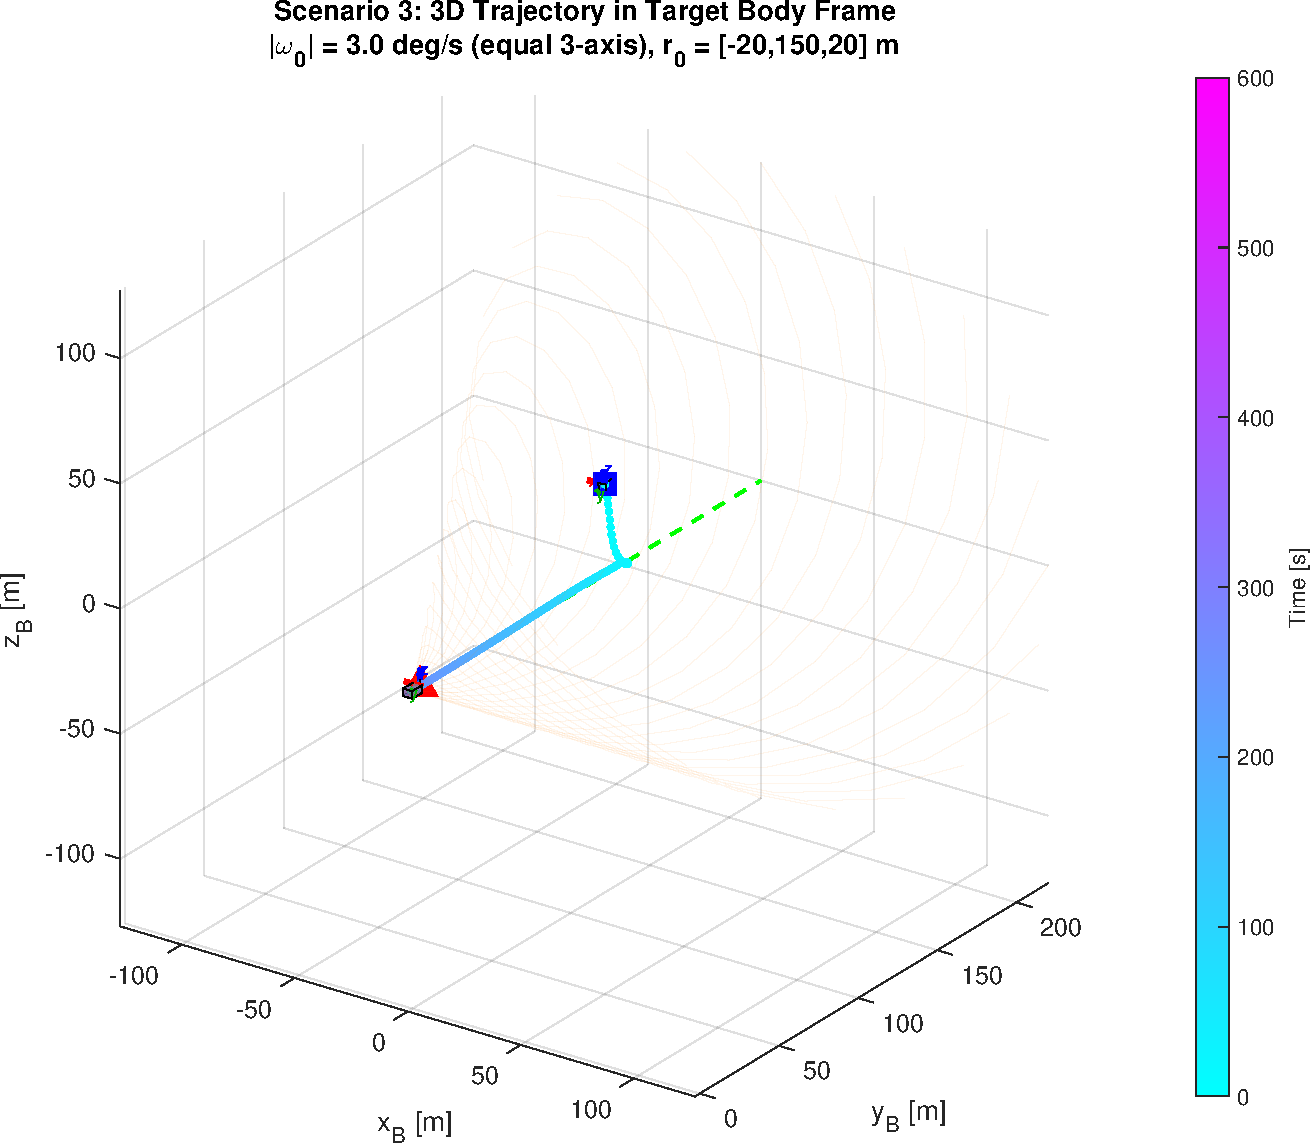
\includegraphics[width=0.95\columnwidth]{fig_3d_trajectory_body.png}
\caption{Chaser trajectory in the target body frame under 3D tumbling
  (intermediate-axis instability, $|\boldsymbol{\omega}_0| = 2.0$~deg/s).
  The colour gradient indicates time progression (blue$\to$pink).
  The orange wireframe shows the $30^\circ$ LOS cone along $+y_B$;
  blue and red markers indicate start and end positions.  The chaser box
  is drawn at start and end with its $+y$ axis pointing toward the target.}
\label{fig:3d_trajectory}
\end{figure}

Figure~\ref{fig:3d_cost} shows the optimal MPC objective value
$J_k^* = \sum_{j=0}^{N_p-1}\bigl[\|\hat{\mathbf{x}}_j - \mathbf{x}^{\mathrm{ref}}_j\|_Q^2 + \|\mathbf{u}_j\|_{R_u}^2 + \|\Delta\mathbf{u}_j\|_{R_{\Delta u}}^2\bigr] + \|\hat{\mathbf{x}}_{N_p} - \mathbf{x}^{\mathrm{ref}}_{N_p}\|_{Q_N}^2$,
evaluated from the QP decision vector $\mathbf{z}^*$ returned by the solver at each control step.
The objective decays over eight orders of magnitude (${\sim}10^6$ to ${\sim}10^{-2}$) as the chaser converges.
The steep initial drop ($t < 80$~s) corresponds to the alignment and corridor-entry phase, after which the trajectory is well within the LOS cone and the objective decreases gradually during the station-keeping phase.

\begin{figure}[H]
\centering
\includegraphics[width=0.95\columnwidth]{fig_cost_history.png}
\caption{Full-horizon MPC objective value $J_k^*$ (log scale) for the 3D tumbling approach, computed from the QP solution at each control step.  The objective includes state-tracking~($Q$), terminal~($Q_N = 30Q$), input~($R_u$), and input-rate~($R_{\Delta u}$) penalties summed over the $N_p = 40$-step prediction horizon.  The cost decays from $\sim\!10^6$ to $\sim\!10^{-2}$ as the chaser converges onto the docking axis.}
\label{fig:3d_cost}
\end{figure}

Figure~\ref{fig:3d_summary} provides a six-panel overview of the approach.
The range tracks the exponential reference trajectory, the LOS margin
remains positive throughout, and the cumulative $\Delta v$ of 32.7~m/s
reflects the additional cost of co-rotating with the tumbling body frame
compared to the planar case.

\begin{figure}[H]
\centering
\includegraphics[width=\textwidth]{fig_summary.png}
\caption{Six-panel summary of the 3D tumbling approach: (a)~range and
  reference, (b)~LOS cone margin (always positive), (c)~angular velocity
  components with axis precession, (d)~body-frame position,
  (e)~control acceleration, (f)~cumulative $\Delta v$.}
\label{fig:3d_summary}
\end{figure}

Figure~\ref{fig:3d_polhode} shows the polhode---the trajectory of
$\boldsymbol{\omega}_B(t)$ in body-frame angular-velocity space.  The
closed orbit on the energy--momentum intersection ellipsoids confirms
classical torque-free rigid-body behaviour and verifies the fidelity
of the Euler-equation integration.

\begin{figure}[H]
\centering
\includegraphics[width=0.75\columnwidth]{fig_polhode.png}
\caption{Polhode trajectory in body-frame $\omega$-space.  The angular
  velocity traces a closed orbit characteristic of intermediate-axis
  instability, confirming conservation of energy and angular momentum.}
\label{fig:3d_polhode}
\end{figure}

\subsubsection{Discussion}

Three key observations emerge from the 3D validation:

\begin{enumerate}
\item \textbf{Body-frame MPC is rotation-agnostic.}  Because the LOS cone
  constraints are defined in the body frame, the MPC formulation requires
  no modification for 3D tumbling.  The rotation complexity is absorbed
  entirely by the Coriolis and centrifugal terms in the linearised dynamics
  \eqref{eq:body_frame_dyn}.

\item \textbf{The synchronisation bound generalises directly.}
  $r_{\mathrm{sync}} = 2a_{\max}/\|\boldsymbol{\omega}_B\|^2 = 330$~m
  for this scenario, and the chaser's initial range (165~m) lies well within
  $r_{\mathrm{sync}}$, consistent with the zero LOS violations observed.
  This confirms the scaling analysis of Section~\ref{sec:reachability}
  for the 3D case.

\item \textbf{$\Delta v$ cost increases with tumble complexity.}
  The 32.7~m/s $\Delta v$ is approximately $2\times$ higher than
  comparable planar cases at the same $|\boldsymbol{\omega}|$ and
  $a_{\max}$, reflecting the additional control effort for
  out-of-plane station-keeping as the body frame rotates about all
  three axes.
\end{enumerate}

The erosion-based analytical certification
(Section~\ref{sec:reachability}) extends to 3D by replacing the planar
rotation velocity $\mathbf{v}_{\mathrm{rot}} = [\omega_t y_B,
-\omega_t x_B, 0]^\top$ with the general cross product
$\mathbf{v}_{\mathrm{rot}} = \boldsymbol{\omega}_B(t) \times
\mathbf{r}_B$.  The erosion formula~\eqref{eq:erosion} remains valid
with this generalised velocity, and the worst-case over the polhode
period provides a conservative bound for the safe-start region.

\subsection{Towards Hamilton--Jacobi Reachability}
\label{sec:hj_discussion}

The erosion-based safe-start region analysis in Section~\ref{sec:reachability}
provides a computationally efficient inner approximation of the true
viability kernel.  A more rigorous characterisation would employ
Hamilton--Jacobi (HJ) reachability analysis~\cite{Mitchell2005,Bansal2017},
which computes the exact backward reachable set (BRS) by solving the
HJ partial differential equation:
\begin{equation}
  \frac{\partial V}{\partial t} + \min\!\bigl[0,\;
  H(\mathbf{x}, \nabla V)\bigr] = 0
\label{eq:hj_pde}
\end{equation}
where $V(\mathbf{x}, t)$ is the value function and $H$ is the Hamiltonian
encoding the dynamics, control authority, and disturbances.  The zero
sublevel set $\{\mathbf{x} : V(\mathbf{x}, t) \le 0\}$ is the exact
viability kernel under optimal control.

For the rotating-corridor problem, HJ reachability would provide:
(i)~the exact safe-start set without the single-step braking
approximation inherent in the erosion model,
(ii)~optimal control policies that maximise the safe region, and
(iii)~formal inclusion guarantees under bounded disturbances.
The primary challenge is computational: HJ scales exponentially with
state dimension, making the full 6D problem ($\mathbf{r}, \mathbf{v}$)
intractable on standard hardware.  Practical approaches include
decomposition into decoupled in-plane/out-of-plane subsystems (4D + 2D)
or projection onto the 2D approach plane ($x_B, y_B$) with velocity
treated parametrically.  Integration of HJ viability kernels with
the YA time-varying dynamics for elliptic orbits is a natural extension
of the framework developed in this paper.


%% ========================================================================
\section{Conclusions}
\label{sec:conclusions}
%% ========================================================================

\begin{enumerate}
\item The analytical hierarchy $\mathcal{X}_{\mathrm{rob}} \subseteq \mathcal{X}_{\mathrm{stoch}} \subseteq \mathcal{X}_{\mathrm{nom}}$ is verified across all 20 parameter combinations with zero point-wise violations.
\item The independent Monte~Carlo set $\mathcal{X}_{\mathrm{MC}}$ validates the analytical predictions but is not analytically nested; MC feasibility can be smaller than nominal at high tumble rates where MPC finite-horizon limitations become significant.
\item $a_{\max}/\omega_t^2$ is the universal scaling parameter for rotating-corridor feasibility.
\item Analytical certification: 53~s vs.\ 2--4~h MC ($\sim$200$\times$ speedup).
\item Nonlinear truth propagation reveals double-integrator artefacts.
\item Approach within $r_{\mathrm{sync}} = 2a_{\max}/\omega_t^2$ achieves zero LOS violations.
\item Extension to elliptic orbits via the Yamanaka--Ankersen STM shows that the erosion-based safe region is invariant to eccentricity at LEO, validating CWH as a conservative baseline.
\item Benchmarking against tube-based robust MPC~\cite{Dong2020,Quartullo2024} and the reachability-guaranteed OCP~\cite{Faraci2025} demonstrates that our erosion-based certification achieves $\sim$34$\times$ speedup over NLP-based methods while providing complementary corridor safety guarantees.
\item Three-dimensional tumbling validation with full Euler dynamics and intermediate-axis instability ($120^\circ$ spin-axis precession) confirms that the body-frame MPC formulation handles arbitrary 3D rotations with zero LOS violations, and that $r_{\mathrm{sync}} = 2a_{\max}/\|\boldsymbol{\omega}\|^2$ generalises directly as the synchronisation bound.
\end{enumerate}

Future work: Hamilton-Jacobi viability kernels for exact safe-set computation, integration with tube-based MPC for online robust tracking, multi-phase approach strategies combining de-tumbling with corridor approach, and navigation uncertainty integration.

\section*{Acknowledgements}

The author thanks the open-source community for the tools used in this work.

\bibliography{acta_references}
\bibliographystyle{elsarticle-num}

\begin{appendices}

\section{CWH State-Transition Matrix}
\label{app:stm}

With $c = \cos(n\tau)$, $s = \sin(n\tau)$:
\begin{equation}
\Phi(\tau) = \begin{bmatrix}
4-3c & 0 & 0 & s/n & 2(1-c)/n & 0 \\
6(s-n\tau) & 1 & 0 & -2(1-c)/n & (4s-3n\tau)/n & 0 \\
0 & 0 & c & 0 & 0 & s/n \\
3ns & 0 & 0 & c & 2s & 0 \\
-6n(1-c) & 0 & 0 & -2s & 4c-3 & 0 \\
0 & 0 & -ns & 0 & 0 & c
\end{bmatrix}.
\end{equation}

\section{Reachability Parameters}
\label{app:params}

\begin{table}[H]
\centering
\caption{Reachability analysis parameters.}
\begin{tabular}{lll}
\toprule
Parameter & Value & Description \\
\midrule
Grid & $300 \times 300$ & Evaluation grid \\
$\alpha$ & 0.05 & Chance constraint prob. \\
$\sigma_{\mathrm{pos}}$ & 0.01 m & Process noise (position) \\
$\sigma_{\mathrm{vel}}$ & $10^{-4}$ m/s & Process noise (velocity) \\
$w_{\mathrm{pos}}$ & 0.05 m & Robust bound (position) \\
$w_{\mathrm{vel}}$ & $5 \times 10^{-4}$ m/s & Robust bound (velocity) \\
$N_{\mathrm{eff}}$ & 50 & Noise accumulation steps \\
\bottomrule
\end{tabular}
\end{table}

\section{Yamanaka--Ankersen State Transition Matrix Derivation}
\label{app:ya_stm}

\subsection{Tschauner--Hempel Equations}
\label{app:TH}

The linearized equations of relative motion on an elliptical reference orbit
are the Tschauner--Hempel (T-H) equations~\cite{TH1965}.  Using true
anomaly $\nu$ as the independent variable instead of time, the in-plane
relative motion satisfies:
\begin{align}
  x'' - 2z' &= 0
  \label{eq:TH_x}\\
  z'' + 2x' - \frac{3}{\rho} z &= 0
  \label{eq:TH_z}
\end{align}
where primes denote differentiation with respect to $\nu$, and:
\begin{equation}
  \rho(\nu) = 1 + e\cos\nu
  \label{eq:rho}
\end{equation}

The out-of-plane motion is decoupled:
\begin{equation}
  y'' + y = 0
  \label{eq:TH_y}
\end{equation}

\noindent The T-H equations reduce to the standard CW (HCW) equations when
$e = 0$ and the independent variable is changed from $\nu$ to time $t$
(with $\nu = nt$ for circular orbits).  Figure~\ref{fig:ya_derivation_flow}
summarises the derivation flow from T-H equations to the full YA-STM.

% --- TikZ: Derivation flowchart ---
\begin{figure}[ht]
\centering
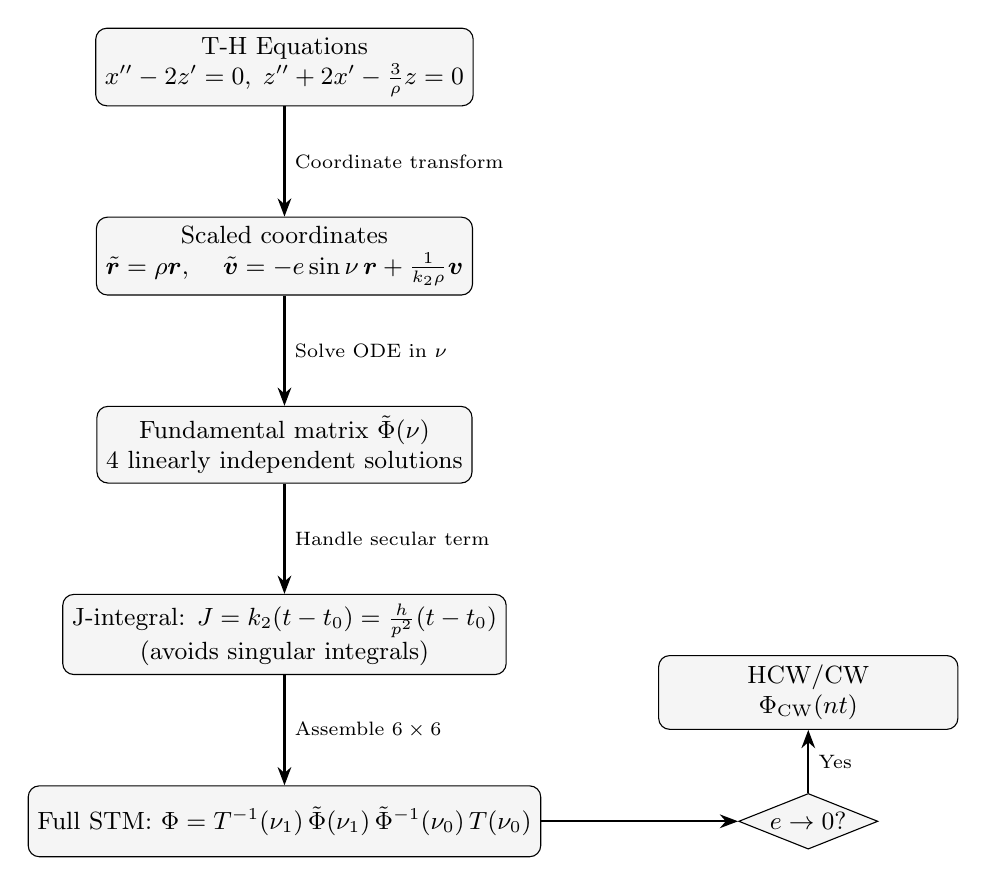
\begin{tikzpicture}[
    node distance=1.4cm,
    block/.style={draw, rounded corners, minimum width=3.8cm,
                  minimum height=0.9cm, align=center, font=\small},
    decision/.style={draw, diamond, aspect=2.5, align=center,
                     font=\small, inner sep=1pt},
    arrow/.style={->,>=Stealth,thick},
]
  % Flow nodes
  \node[block,fill=gray!8] (TH)
    {T-H Equations\\$x''-2z'=0,\; z''+2x'-\frac{3}{\rho}z=0$};
  \node[block,fill=gray!8,below=of TH] (scaled)
    {Scaled coordinates\\$\tilde{\vect{r}}=\rho\vect{r}$, \quad
     $\tilde{\vect{v}}=-e\sin\nu\,\vect{r}+\frac{1}{k_2\rho}\vect{v}$};
  \node[block,fill=gray!8,below=of scaled] (fund)
    {Fundamental matrix $\tilde{\Phi}(\nu)$\\4 linearly independent solutions};
  \node[block,fill=gray!8,below=of fund] (Jint)
    {J-integral: $J = k_2(t-t_0) = \frac{h}{p^2}(t-t_0)$\\(avoids singular integrals)};
  \node[block,fill=gray!8,below=of Jint] (STM)
    {Full STM: $\Phi = T^{-1}(\nu_1)\,\tilde{\Phi}(\nu_1)\,
     \tilde{\Phi}^{-1}(\nu_0)\,T(\nu_0)$};

  % Decision
  \node[decision,right=2.5cm of STM,fill=gray!8] (check)
    {$e \to 0$?};
  \node[block,fill=gray!8,above=0.8cm of check] (HCW)
    {HCW/CW\\$\Phi_{\text{CW}}(nt)$};

  % Arrows
  \draw[arrow] (TH) -- (scaled)
    node[right,font=\scriptsize,midway] {Coordinate transform};
  \draw[arrow] (scaled) -- (fund)
    node[right,font=\scriptsize,midway] {Solve ODE in $\nu$};
  \draw[arrow] (fund) -- (Jint)
    node[right,font=\scriptsize,midway] {Handle secular term};
  \draw[arrow] (Jint) -- (STM)
    node[right,font=\scriptsize,midway] {Assemble $6\times 6$};
  \draw[arrow] (STM) -- (check);
  \draw[arrow] (check) -- (HCW)
    node[right,font=\scriptsize,midway] {Yes};
\end{tikzpicture}
\caption{Derivation flow for the Yamanaka--Ankersen State Transition Matrix.
The key innovation is the J-integral, $J = k_2(t - t_0)$, which replaces
the singular integrals present in earlier T-H solutions.}
\label{fig:ya_derivation_flow}
\end{figure}

\subsection{Scaled Coordinates}
\label{app:scaled}

Yamanaka and Ankersen~\cite{Yamanaka2002} introduced scaled (``tilde'')
coordinates that transform the T-H equations into a form admitting a
closed-form fundamental matrix.  Define:
\begin{align}
  \tilde{\vect{r}} &= \rho\,\vect{r}
  \label{eq:r_tilde}\\
  \tilde{\vect{v}} &= -e\sin\nu\,\vect{r} + \frac{1}{k_2\rho}\,\vect{v}
  \label{eq:v_tilde}
\end{align}
where $k_2 = h/p^2$ with $h = \sqrt{\mu p}$ the specific angular momentum
and $p = a(1-e^2)$ the semi-latus rectum.

In matrix form, the coordinate transformation is:
\begin{equation}
  \begin{bmatrix} \tilde{\vect{r}} \\ \tilde{\vect{v}} \end{bmatrix}
  = \mat{T}(\nu)
  \begin{bmatrix} \vect{r} \\ \vect{v} \end{bmatrix},
  \qquad
  \mat{T}(\nu) =
  \begin{bmatrix} \rho\,\mat{I}_3 & \mat{0}_3 \\
                  -e\sin\nu\,\mat{I}_3 & \frac{1}{k_2\rho}\mat{I}_3
  \end{bmatrix}
  \label{eq:T_transform}
\end{equation}

\subsection{Fundamental Matrix}
\label{app:fund_matrix}

In the scaled coordinates, the in-plane fundamental matrix columns are
constructed from four linearly independent solution vectors.  Define the
auxiliary functions:
\begin{align}
  s(\nu) &= \rho\sin\nu & c(\nu) &= \rho\cos\nu
  \label{eq:s_c}\\
  s'(\nu) &= \cos\nu + e\cos 2\nu & c'(\nu) &= -(\sin\nu + e\sin 2\nu)
  \label{eq:sp_cp}
\end{align}

The $4 \times 4$ in-plane fundamental matrix at true anomaly $\nu$
(in the paper's $[x, z, \dot{x}, \dot{z}]$ ordering) is:
\begin{equation}
  \tilde{\Phi}_{\text{ip}}(\nu, J) =
  \begin{bmatrix}
    1 & -c(1+\rho^{-1}) & s(1+\rho^{-1}) & 3\rho^2 J \\[4pt]
    0 & s & c & 2 - 3esJ \\[4pt]
    0 & 2s & 2c - e & 3(1 - 2esJ) \\[4pt]
    0 & s' & c' & -3e(s'J + s/\rho^2)
  \end{bmatrix}
  \label{eq:Phi_tilde_ip}
\end{equation}

The J-integral that appears in the fourth column is:
\begin{equation}
  \boxed{J = k_2(t - t_0) = \frac{h}{p^2}(t - t_0)}
  \label{eq:J_integral}
\end{equation}
This is the central innovation of the Yamanaka--Ankersen formulation.
Previous T-H solutions~\cite{Carter1998} required evaluation of the
integral $\int_{\nu_0}^{\nu_1} \frac{d\nu}{\rho^2(\nu)}$, which has no
simple closed form for $e \neq 0$.  The key insight is that this integral
equals $k_2\,\Delta t$, which can be computed directly from the elapsed
time without evaluating the integral.

The out-of-plane $2\times 2$ block is a simple rotation by $\Delta\nu$:
\begin{equation}
  \tilde{\Phi}_{\text{oop}}(\Delta\nu) =
  \begin{bmatrix}
    \cos\Delta\nu & \sin\Delta\nu \\
    -\sin\Delta\nu & \cos\Delta\nu
  \end{bmatrix}
  \label{eq:Phi_oop}
\end{equation}

\subsection{Full STM Assembly}
\label{app:stm_assembly}

The complete $6\times 6$ STM in physical coordinates is assembled as:
\begin{equation}
  \boxed{
  \Phi(\nu_0 \to \nu_1) =
  \mat{T}^{-1}(\nu_1)\;\tilde{\Phi}(\nu_1,J)\;
  \tilde{\Phi}^{-1}(\nu_0, 0)\;\mat{T}(\nu_0)
  }
  \label{eq:full_STM}
\end{equation}
where $\tilde{\Phi}^{-1}(\nu_0, 0)$ is the inverse of $\tilde{\Phi}$
evaluated at $\nu_0$ with $J = 0$ (see Figure~\ref{fig:stm_structure}
for the block structure).  The inverse transform is:
\begin{equation}
  \mat{T}^{-1}(\nu) =
  \begin{bmatrix}
    \frac{1}{\rho}\,\mat{I}_3 & \mat{0}_3 \\[4pt]
    k_2 e\sin\nu\,\mat{I}_3 & k_2\rho\,\mat{I}_3
  \end{bmatrix}
  \label{eq:T_inv}
\end{equation}

% --- TikZ: STM block structure ---
\begin{figure}[ht]
\centering
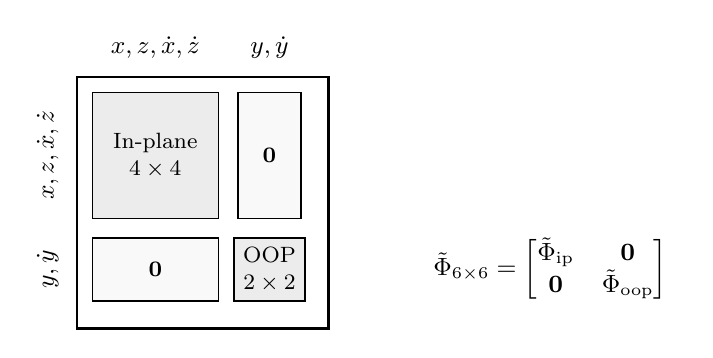
\begin{tikzpicture}[
    block/.style={draw, minimum width=1.6cm, minimum height=1.6cm,
                  align=center, font=\footnotesize},
    >=Stealth,
]
  % 6x6 grid
  \node[block,fill=gray!15] (A) at (0,0) {In-plane\\$4\times 4$};
  \node[block,fill=gray!5,minimum width=0.8cm] (B) at (1.45,0) {$\mat{0}$};
  \node[block,fill=gray!5,minimum height=0.8cm] (C) at (0,-1.45) {$\mat{0}$};
  \node[block,fill=gray!15,minimum width=0.8cm,minimum height=0.8cm] (D) at (1.45,-1.45)
    {OOP\\$2\times 2$};

  % Labels
  \node[above=0.3cm of A,font=\small] {$x,z,\dot{x},\dot{z}$};
  \node[above=0.3cm of B,font=\small] {$y,\dot{y}$};
  \node[left=0.3cm of A,font=\small,rotate=90,anchor=south] {$x,z,\dot{x},\dot{z}$};
  \node[left=0.3cm of C,font=\small,rotate=90,anchor=south] {$y,\dot{y}$};

  % Overall label
  \node[right=1.5cm of D,font=\small,align=left] (eq) {
    $\tilde{\Phi}_{6\times 6} = \begin{bmatrix}
    \tilde{\Phi}_{\text{ip}} & \mat{0} \\
    \mat{0} & \tilde{\Phi}_{\text{oop}}
    \end{bmatrix}$
  };

  % Brace
  \draw[thick] (-1.0,1.0) rectangle (2.2,-2.2);
\end{tikzpicture}
\caption{Block structure of the YA-STM fundamental matrix in scaled
coordinates. The in-plane $4\times 4$ block couples the
along-track--radial dynamics; the out-of-plane $2\times 2$ block is
a decoupled rotation.}
\label{fig:stm_structure}
\end{figure}

\end{appendices}

\end{document}
